\ifdefined\BuildingFromMainFile
\else
   \documentclass[../main.tex]{subfiles}
   \begin{document}
\fi


\graphicspath{{figure/}{../figure/}}

\newpage
\onehalfspacing

\linespread{1.25}
\setlength{\parskip}{\baselineskip}

\normalsize

\section{Genomic technologies to assess genetic variations in livestock}

Cattle is an important livestock species for producing animal-based protein. The global cattle population is highly diverse due to intense selection for specific breeding goals, such as for production of milk, beef, or both (dual-purpose), as well as the adaptation to a wide range of environments \citep{zhang2020evolution}. Due to selective breeding and improved husbandry conditions, spectacular increases in livestock productivity have been achieved. For example, the average annual milk yield per cow in the United State has increased by more than five-fold from 1,890 kg in 1924 to 9,682 kg in 2011 \citep{georges2019harnessing}. 

Genomic selection had been proposed to further accelerate genetic gain \citep{meuwissen2001prediction}. To this end, the genetic value of an individual is estimated based on genome-wide molecular marker information. Genotyping arrays were first developed to assess variation at thousands of polymorphic sites in the genome. The genotype information is then linked to phenotype to determine markers associated with agriculturally-important traits \citep{goddard2009mapping} or to derive the prediction equation for genomic selection \citep{meuwissen2001prediction}. More than 3 million cattle in the USA have already been genotyped \citep{wiggans2017genomic}. However, variations covered by chip-based genotyping  are  not comprehensive enough  to pinpoint causal mutations underlying the traits \citep{pausch2017evaluation}.

This limitation prompted the utilization of whole-genome sequencing based on the short-read sequencing technology. In this approach, the DNA is first fragmented and subsequently read-out in segments of few hundred bases (Fig. \ref{fig11:reseq}). Variation discovery typically follows a reference-guided alignment approach. Genotypes are called at positions where the observed nucleotides from the alignments differ from the corresponding reference nucleotides. Sophisticated variant calling algorithms were developed to differentiate between real variants and sequencing errors from noisy short-read data or misalignments \citep{depristo2011framework}. Whole genome sequencing approaches can accurately discover small variants (SNPs and Indels < 50 bp) across the whole genome. 

Sequencing costs have dropped substantially over the past decades, faster than Moore’s Law (a term in computer hardware that doubling power every two years indicates a well-progressed technology), which has paved the way towards sequencing a genome for only \$100 \citep{Regalado2020,Wetterstrand2020}. The decline in sequencing costs has also enabled the sequencing of individual cattle genomes for agricultural applications. The 1000 Bull Genome Project was launched to coordinate global sequencing efforts and compile huge datasets.  In their latest  (8$^{th}$ ) run, the consortium has already catalogued more than 150 million variants from more than 3500 cattle acrossf 200 breeds \citep{hayes20191000}. This variant database has become a powerful resource to impute sequence variant genotypes into large mapping cohorts, thus accelerating the discovery of causal mutations  for complex and monogenic traits and improve the prediction accuracy of genomic selection \citep{daetwyler2014whole}. Recently, low-pass sequencing (<1x) coupled with genotype imputation techniques were proposed as a cost-effective strategy to enable population-scale whole genome sequencing variant analysis \citep{snelling2020assessment}. \\

\bigskip

\begin{figure}[!htb]
    \centering
    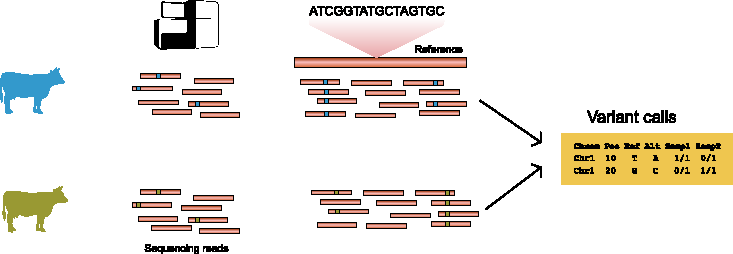
\includegraphics[width=\textwidth]{intro/fig1.pdf}
        \vspace{3mm}
        \caption[Identification of genetic variants through re-sequencing]{\textbf{Identification of genetic variants through re-sequencing} \\
        \footnotesize{Whole-genome sequences were fragmented into billions of short fragments which were then read by DNA sequencer in a massively parallel manner. The sequencing reads were compared (aligned) to the reference genome. Genetic variants were identified as nucleotide discordances relative to the reference sequences.}}
        \label{fig11:reseq}
\end{figure}


\section{Improvements in the cattle reference genome} 

A well-annotated reference genome is the starting point for many genomic analyses. It serves as a reference point for read alignments, variant calling, gene annotation, and functional analysis. Gene loci are defined at specific genomic coordinates, and alleles are referred to as alternative or reference  nucleotides. The ability to compare billions of sequencing reads from hundreds to thousands of individuals to the reference sequences has quickly become the gold standard, identifying variants underpinning  inherited diseases or other relevant traits, thus accelerating genetic progress \citep{bickhart2020symposium}.

The first cattle reference genome (Btau 3.1 and Btau 4.0) was assembled in 2009 from  sequencing reads from bacterial artificial chromosome (BAC) and whole-genome shotgun (WGS) sequencing \citep{elsik2009genome}. The contig and scaffold N50 for this assembly were 48.7 kb and 1.9 Mb respectively. This assembly was further refined in 2014 to close gaps and correct structural errors (UMD\_3.1.1) using additional sequencing data and sophisticated assembly approaches \citep{zimin2009whole}. The most recent cattle reference genome (ARS-UCD 1.2) was assembled from single-molecule real-time (SMRT) long-read sequencing data and scaffolded with optical mapping. The quality of the resulting assembly improved considerably over UMD3.1 with contig and scaffold N50 values of 25.89 Mb and 103 Mb, respectively \citep{rosen2020novo}. Advances in assembly techniques (e.g., trio binning) and the development of highly accurate long-read sequencing technology now enable the construction of assemblies of high continuity, correctness and completeness \citep{bickhart2020symposium}. The recently generated assemblies exceed in quality the current bovine reference genome with contig N50 exceeding 70 Mb and could resolve complex genomic regions, e.g. major histocompatibility regions \citep{rice2020continuous}. Trio binning takes advantage of the high heterozygosity in hybrids to separate long reads according to parental origins. The assembly is subsequently performed separately from the partitioned reads resulting in two haplotype-resolved assemblies. This approach  was first applied  to a cross between Bos taurus x Bos indicus cattle (Angus x Brahman) \citep{koren2018novo}, but now has been applied to broad range cattle breeds, including  undomesticated and/or cattle relatives (Yak, Gaur, Bison) \citep{oppenheimer2021reference}. Recently, the Bovine Pangenome Consortium \citep{heaton2021reference} was initiated to coordinate genome assembly efforts and characterize the complete diversity from hundreds of global cattle breeds, including the wild-relatives and under-represented breeds. 

\section{One reference genome is not enough}

\subsection{A single linear genome cannot fully represent species diversity}

Despite recent spectacular quality improvements, the linear reference genomes are still a poor representation of the full genomic diversity of a species. A linear reference genome represents only one mosaic haplotype of either one or a few individuals. For example, the current cattle reference genome (ARS-UCD1.2) was assembled from a DNA sample from a single highly-inbred animal from the Hereford breed named Dominette, which was initially selected to simplify the assembly process \citep{rosen2020novo}. Reference assemblies from  other livestock species were generated using a similar approch, e.g., Duroc breed used for Sscrofa11.1 pig reference \citep{warr2020improved}, San Clemente breed for domestic goat reference \citep{bickhart2017single}, and boxer breed for  CanFam 3.1 dog reference \citep{lindblad2005genome}. While the selection of reference animals seems to be trivial, the resulting reference sequences do not necessarily reflect the most common allele in the population or from samples with the most ideal phenotypes \citep{ballouz2019time}. Reference-guided variant discovery might reflect some properties of the reference animal rather than the population; e.g., variant calling will output more variants when the reference  contains rare alleles. \citet{low2019haplotype} found a striking difference in the number of polymorphic sites when calling Angus variants from an Angus reference than from a Brahman reference. Additionally, the reference genome might carry the lower frequency variants or variants private to the reference animals. \citep{shukla2019hg19kindel,ballouz2019time} estimated that 2 million bases in the human reference genome are minor alleles. 

\subsection{Insufficient representation of linear genomes cause reference bias}

Because the alignment algorithms compare the reads towards the reference and try to minimize differences, the reference-guided variant discovery will always be biased towards the reference bases. In other words, it is easier to align DNA fragments without differences to the reference bases than DNA fragments  that contain non-reference bases. Comparison of the sequencing reads with variants, even if they are the true representation of that species, will be penalized, resulting in sub-optimal alignments, misalignments, or cannot be mapped (Fig. \ref{fig12:bias}) \citep{pritt2018forge}. Together, this limitation is referred to as \textbf{soft reference bias}, which hampers genomic analysis that depends on the allelic balance such as heterozygous variant calling \citep{garrison2018variation}, allelic-specific expression \citep{salavati2019elimination}, or analysis in the highly polymorphic regions \citep{dilthey2015improved}. \citet{wu2018pervasive} observed the impact of reference bias affecting a lower estimate of divergence among Bos species due to mapping of cattle-relatives data to the Bos taurus reference genome, which tends to overlook the diverged regions. 

Another limitation is referred to as \textbf{hard reference bias}, whereby a single reference is a poor representation of large structural variations that diverged between individuals in the population (Fig. \ref{fig12:bias}) \citep{colquhoun2020nucleotide}. Reads originating from these highly diverged segments will remain unmapped and all subsequent genomic analyses will be blind to variations in these “missing” regions. In cattle, the comparison between two taurine assemblies revealed 10.9 Mb of Angus-specific sequences that were not present in the Hereford-based reference assembly \citep{low2019haplotype}. This number increases to 21.8 Mb when the Angus assembly is compared to an indicine cattle genome. Reference genomes lacking millions of bases has been observed in many species. \citet{ameur2018novo,audano2019characterizing} estimated that each human genome on average carries about 10 Mb non-reference bases. Long read data analysis across global ancestries discovered 8.5 Mb insertions observed in majority of the human population \citet{audano2019characterizing}. Remarkably, an analysis of the unmapped reads of the African pangenome revealed 300 Mb non-reference insertions, suggesting that the existing human reference genome might lack diversity spanning 10\% of the genome (Sherman et al. 2019). \\

\bigskip

\begin{figure}[!htb]
    \centering
    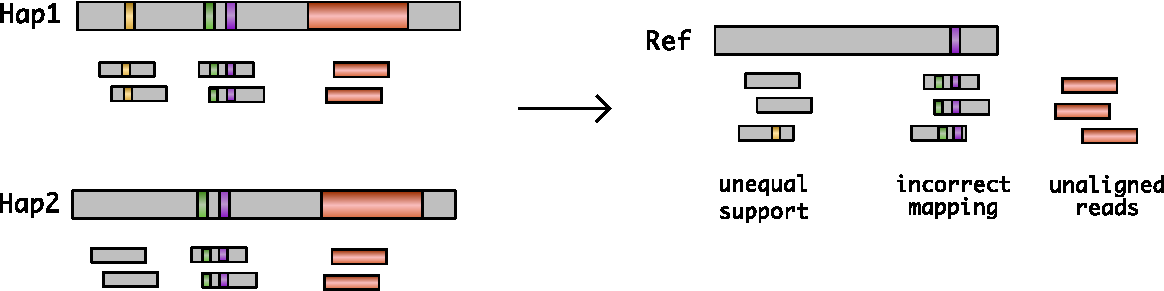
\includegraphics[width=\textwidth]{intro/fig2.pdf}
        \vspace{3mm}
        \caption[Illustration of the reference allele bias]{\textbf{Illustration of the reference allele bias.} \\
        \footnotesize{The origin of short sequencing reads of the sample (hap1 and hap2) are determined by alignments to the reference nucleotides. Thus, the comparison will always be biased towards nucleotides in the reference. Alignment of reads with alleles differing from reference might receive lower support than allele matches to the reference nucleotides (yellow stripe), results in incorrect alignments with multiple variations (green and purple stripes), or remain unmapped if the regions not present in the reference (e.g., large insertion, orange box). Grey background denotes reference sequences.}}
        \label{fig12:bias}
\end{figure}

\subsection{The problem of reference bias is magnified in a species with high genetic diversity}

The effect of reference bias will be more pronounced in a highly diverged species like in cattle. Genetic architecture of the bovine genomes has been shaped by various processes related domestication, admixture, introgression, local adaptation, and human-directed selection \citep{zhang2020evolution}, resulting in the creation of more than 600 subpopulation (known as breeds) adapted for a variety of environmental conditions and selected for various breeding goals. Genetic diversity is higher in cattle than human populations \citep{charlier2016ngs}. The bovine species formed the bovine tribe which subdivided into three sub-tribes diverged about 10-15 million years ago: the \emph{Pseudorygina},\emph{ Bubalina} (Buffalo), and \emph{Bovina} (genus Bison and Bos). Specifically, the subtribe bovina is comprised of three subtribes split about 3-5 million years ago: (i) yak, bison; (ii) gaur,gayal, and banteng; and (iii) taurine and zebu \citep{pitt2019domestication}. Generally, Taurine breeds (\emph{Bos taurus taurus}) are intensively selected for production traits (milk and beef) and have higher fertility than indicine breeds. Indicine breeds (\emph{Bos taurus indicus})  generally have lower production traits and fertility, but still possess desirable traits related to heat tolerance, parasite and disease resistance \citep{low2019haplotype}. However, these characteristics are not strict as there are numerous local cattle breeds optimized for specialized breeding goals \citep{signer2017population,upadhyay2019genomic}. Series of introgressions and hybridizations created specialized breeds with mosaic genomes, such as Brahman, composed of ~10 \% taurine and 90\% indicine origin \citep{koufariotis2018sequencing}. African cattle are generally admixture between \emph{Bos taurus} x \emph{Bos indicus}, where the introgressed regions are selected for African pastoralism \citep{kim2020mosaic}. On average, each individual cattle carry more than 5 million variants relative to Bos taurus reference, which is higher than variations reported in the human population at about 3-4 million variants \citep{daetwyler2014whole,sudmant2015integrated}. The number of variants is higher in more diverged, indicine \citep{koufariotis2018sequencing} or under-studied African cattle \citep{kim2020mosaic,kim2017genome}. Additionally, this amount likely underestimates the actual genetic diversity as it does not consider the structural variations, which are poorly characterized with short-read sequencing technology \citep{mahmoud2019structural,chaisson2019multi}. 

\section{Strategies to mitigate reference bias}

\subsection{Modification of the existing linear reference genome}

Some strategies have been proposed to mitigate the reference bias. The most straightforward solution is to create a so-called consensus reference genome, whereby each minor allele in the reference sequence is replaced by the most frequent allele in the population. Since the transformed reference is still in the linear space, the downstream genetic analysis can still use the tools currently developed for linear genomes. However, a coordinate lift-over is needed when indels are included in the substitutions. \citet{ballouz2019time} built consensus human reference by replacing 2 million minor alleles with the corresponding major allele, that reduced mapping error by a factor of three and improved the quantification of transcripts \citep{kaminow2020virtue}. \citet{chen2021reference} extended this idea into a so called reference flow approach, whereby it re-aligned sub-optimally mapped reads into a set of genomes from multiple population, that could reduce strongly heterozygous sites by 22\%. Another effort, as in the human genome, is by continually expanding reference with alternative contigs in the polymorphic regions that are impossibly represented with a single haplotype. There were currently 13 updates with 261 alternate patches that add 109 Mb total length. However, this strategy is not sustainable with more diversity included. Additionally, the lack of tools that can properly handle these additional overlapping contigs will likely not be able to mitigate the reference bias \citep{sherman2020pan}. 

\subsection{Creation of population-specific genome assemblies}

The reduced cost of long-read sequencing and improved assembly techniques  make it easier to generate high-quality, near error-free, and complete genome assemblies \citep{miga2020telomere,logsdon2021structure}. Thus, more studies have now shifted from species-level references into population-specific reference genomes, effectively creating more personalized genomes. Large genomic initiatives such as Vertebrate Genome Project (VGP, \url{https://vertebrategenomesproject.org/}), Darwin Tree of Life (\url{https://www.darwintreeoflife.org/}), or Earth Bio-genome Project \citep{lewin2018earth} contributes to the explosion the number of genome assemblies across the tree of life accessible in the public domain. The first phase of VGP generated 268 vertebrate genomes using long-read data, that further scaffolding with optical mapping results in the chromosome-scale assemblies and fulfilling the strict high-quality criteria \citep{rhie2020towards}. On the other hand, some genomic initiatives focus to deeply characterize the diversity of a single species, such as the Human Pangenome Reference Consortium (HPRC) that plans to generate 350 human assemblies representing global ancestries (see \url{https://humanpangenome.org/}). A similar internationally coordinated effort was also initiated for cattle with the Bovine Pangenome Consortium \citep{heaton2021reference} that aim to generate reference-quality assemblies across global cattle breeds. There are already dozens of genomes from livestock species publicly available in NCBI assembly. As in other species, the application of third generation sequencing technology results in an outstanding improvement in assembly quality. This was pioneered with goat genome that improved the contiguity over 400 times compared to the previous short-read based assembly \citep{bickhart2017single}. As of April 2021, there are chromosome-level assemblies of 22 cattle (\emph{Bos}) and its relatives (gaur, gayal, yak, bison), 19 pigs (\emph{Sus}), 7 sheeps (\emph{Ovis}), 4 goats (\emph{Capra}), 9 dogs (\emph{Canis}), with many more continuing to be added.

\section{Transition from genomics to pangenomics}

\subsection{Definition of the pangenome}

Accumulating evidence suggests that a single genome cannot represent  the full diversity of a species, motivating the development of  pangenomes. A pangenome refers to a structure used to  integrate multiple genomes, reflecting the complete species diversity rather than collapsing all variations into a single haplotype, see recent reviews \citep{bayer2020plant,golicz2016pangenome,sherman2020pan,della2021pan}. The term pan-genome (pan – whole, Greek) was first introduced by \citet{tettelin2005genome} to describe complete gene repertoire across Streptococcus agalactiae strains where 20\% of the genes are variable across isolates. This concept was quickly adopted across the tree of life, including the agriculturally important plant and animal species, such as pig \citep{li2017comprehensive,tian2019building}, goat \citep{li2019towards}, and human \citep{duan2019hupan,sherman2019assembly}. There has been rapid growth in the number of pangenome publications across years \citep{bayer2020plant}, with close to 8000 studies indexed by PubMed,  although most currently focus on bacterial pangenomes.  

\subsection{Categorization of the pangenome}

The content of a pangenome may be divided into the core and flexible genome (also known  as dispensable or accessory genome, Fig. \ref{fig13:pan}a). Core genome is common sequences across all individuals that is responsible for maintaining essential function (e.g., DNA replication, cellular homeostasis and cellular processes). This part of genomes is under purifying selection, thus having less diversity. Dispensable genomes are segments that vary across individuals. They are under less evolutionary constraint, which allows for contributions to numerous adaptive phenotypes, mainly disease, biotic, and abiotic resistance, survival, immunity, defence response, adaptation to new environments, communications, and signalling \citep{golicz2020pangenomics}. Thus, dispensable genomes are of particular interest for the studies of adaptive traits that might drive genetic differentiation and give population their distinguishing characteristics. In animals, the pangenome is largely dominated by core component (e.g., 96.67\% of genes in the human) \citep{duan2019hupan}. However, a recent report in the Mediterranean mussel Mytilus galloprovincialis, with high-stress tolerance and lineage-specific duplications, indicates that up to 25\% of the total genome is variable \citep{gerdol2020massive}. Pangenomes have been extensively characterized in plants, among them are in rice \citep{zhao2018pan}, tomato \citep{gao2019tomato}, wheat \citep{walkowiak2020multiple}. They reported larger proportion of accessory genomes (>20\%), particularly in polypoid, outcrossing, or species history of whole-genome duplications \citep{tao2019exploring}. Higher ratio of flexible to core genome indicates a species with higher adaptability \citep{tranchant2018plant}. 

It is important to consider whether the pangenome is of either closed or open type. In a closed type pangenome, the sequencing of sufficient samples will capture the whole pangenome, and thus the size of the complete pangenome can be computationally predicted. On the other hand, sequencing more individuals will recover more pangenome content in an open pangenome. Thus, the size of pangenome keeps increasing as more samples included \citep{golicz2020pangenomics}. Many plant and animal pangenomes are a closed type in terms in the number of genes but open in terms of total sequence content \citep{duan2019hupan,golicz2020pangenomics}, which also suggests that the non-coding segments primarily drive the sequence variability across samples. Bacterial pangenomes  are generally open due to prevalence of horizontal gene transfer \citep{soucy2015horizontal}. Sampling bias of underrepresented diversity (such as genetically related samples) could lead to the falsely concludingthe pangenome is complete \citep{tranchant2018plant}. With additional, sufficiently  diverged samples, the  pangenome would continue to grow. Thus, sampling strategy in a pangenome study should maximize diversity to fully retrieve the complete pangenome. 

\begin{figure}[!htb]
    \centering
    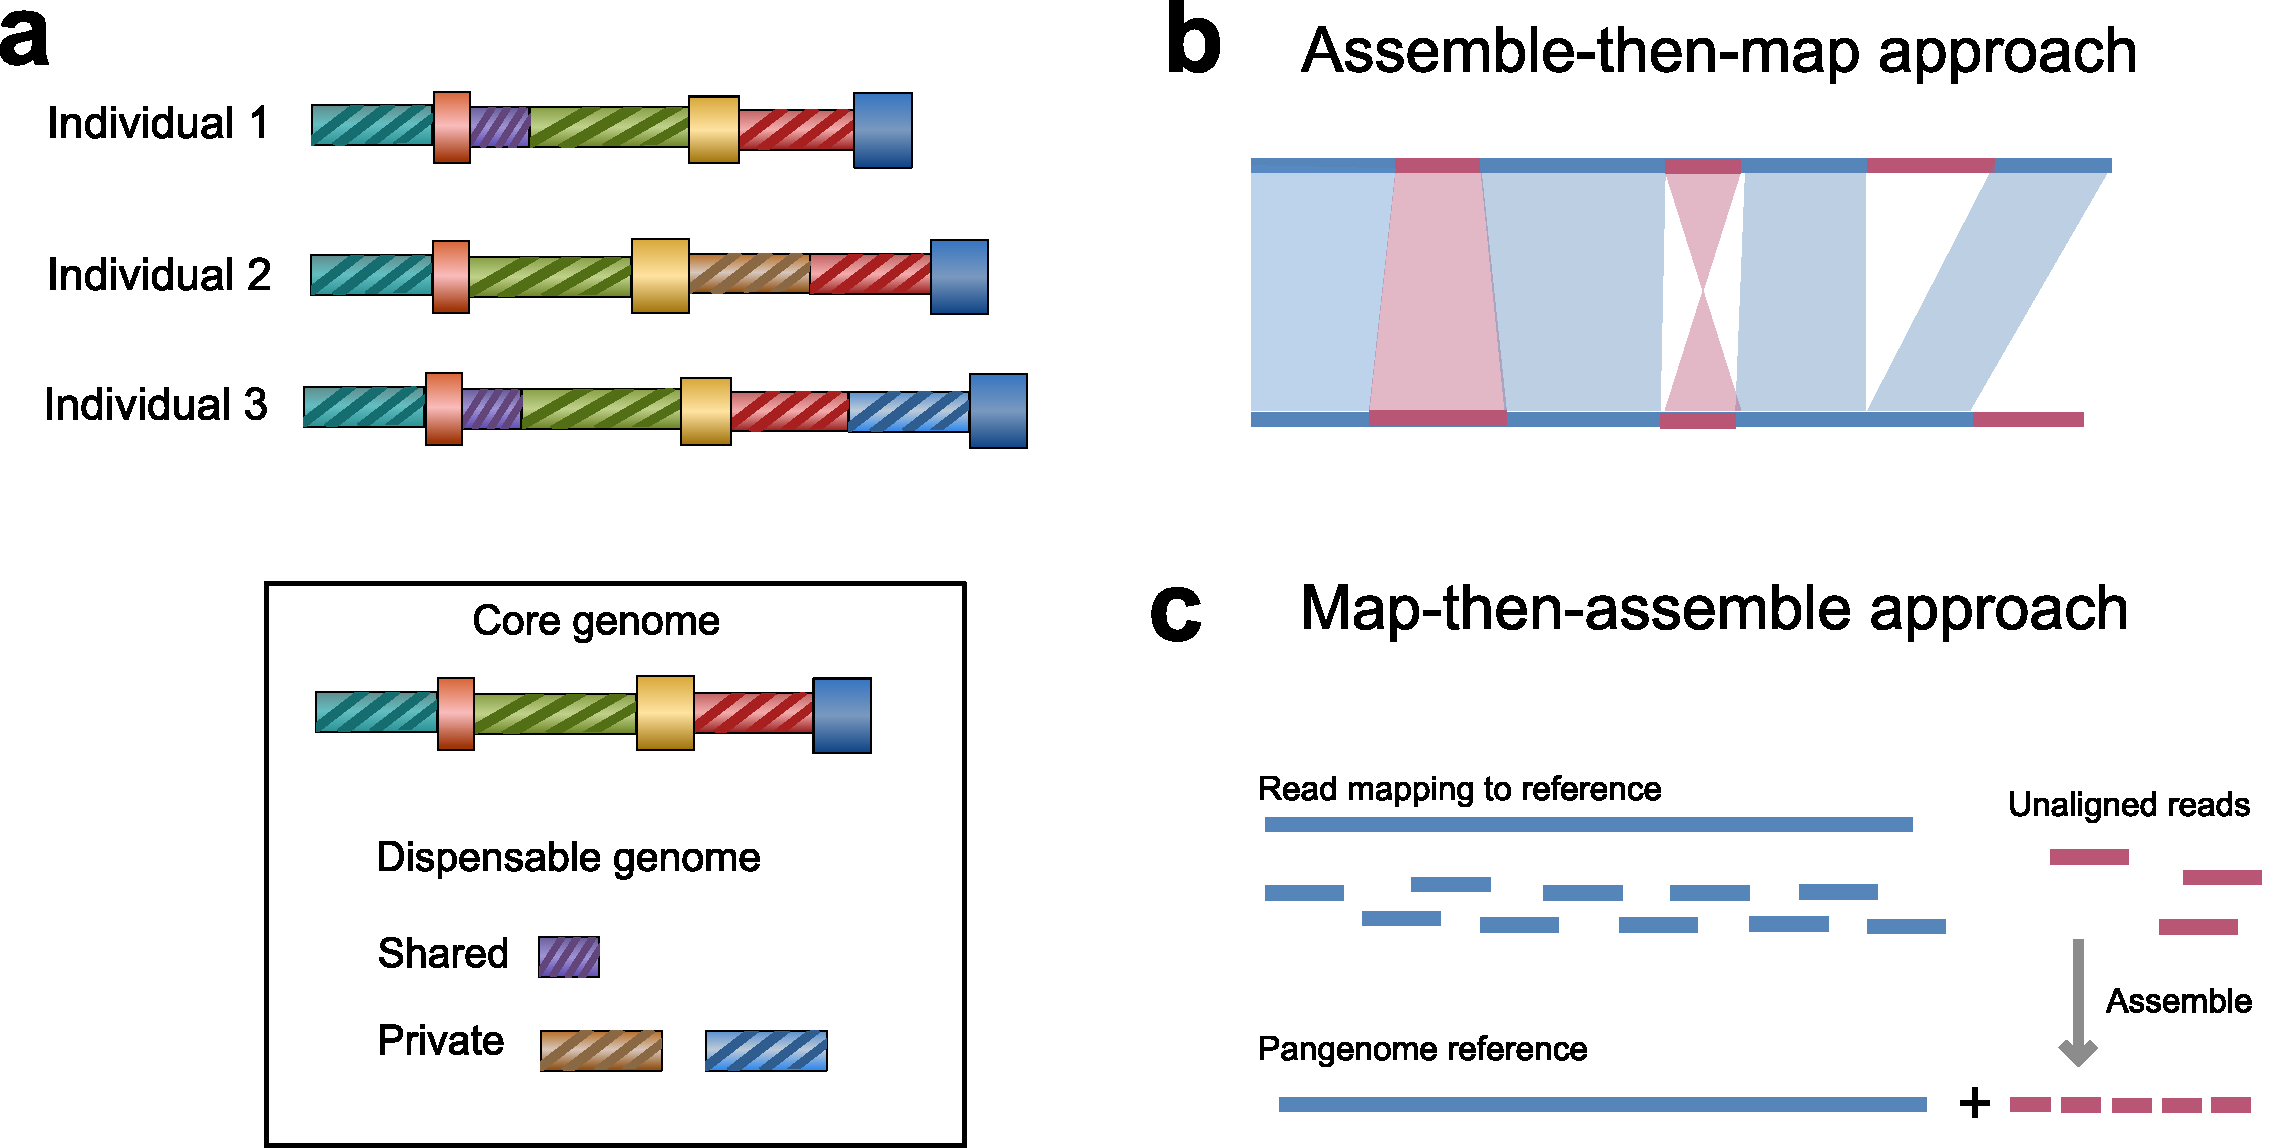
\includegraphics[width=\textwidth]{intro/fig3.pdf}
        \vspace{3mm}
        \caption[The concept of pangenomes]{\textbf{The concept of pangenomes.} \\
        \footnotesize{\textbf{(a)} Pangenomes refers to a collection of individual genomes in the populations, which is further divided into core (shared by all members of populations) and flexible parts that the presence varies across individuals. Different strategies to build the pangenome \textbf{(b)} Assemble-then-map: Genomes from multiple individuals are assembled, which are then compared to the reference assembly \textbf{(c)} Map-then-assemble: sequencing reads from multiple individuals are aligned into the reference. Unmapped sequences assembled and added as additional contigs to the reference sequences. Figures are adapted from \citep{sherman2020pan} and \citep{bayer2020plant}.}}
        \label{fig13:pan}
\end{figure}


\subsection{Approaches building the pangenome}

There are two commonly used approaches to build a pangenome (Fig. \ref{fig13:pan}bc): “assemble-then-map" and “map-then-assemble" (also known as map-to-pan) \citep{golicz2020pangenomics}. In the “assemble-then-map"-strategy, each genome is assembled and annotated independently, which is then followed by pairwise alignment of all assembled genomes to determine shared and non-shared segments \citep{duan2019hupan,li2019towards,eisfeldt2020discovery}. This assembly-based strategy is supposed to recover the full-length non-reference sequences and resolve repetitive and complex structural variants. However, this approach depends on the assembly contiguity and completeness. Assembly and annotation errors make the comparison difficult and may lead to erroneous identification of the structural variations. Additionally, genome assemblies are still too expensive to be performed on the population-scale, limiting analysis only on a subset of individuals. To take advantage the massive amount of population-scale of the short-read sequencing data, the majority of  recent pangenome studies utilize the “map-then-assemble"-approach \citep{holden2018assembly,laine2019exploring,sherman2019assembly}. Sequencing reads from each sample are independently mapped to the reference genome. The  unmapped (or poorly mapped) reads are subsequently assembled to obtain the non-reference sequences. However, due to the nature of short-read-based assembly, most of the resulting contigs are fragmented, making it difficult to locate the breakpoints’ origins in the reference genome \citep{sherman2019assembly}. 

\section{Graph-based pangenomics}

\subsection{Graphs as richer reference structures to integrate the genetic diversity}

The pangenome approaches based on unmapped reads or assembly comparison, as discussed above, rely on collections of linear genomes and do not attempt to provide coherent representation that relates all genomes. Considering the prevalence of genetic variations across individuals in the population and availability of abundant genomic resources, the linear representation is clearly an oversimplification. Emerging pangenome methods are developed to build richer variation-aware reference structures that unify the complete genetic diversity of a species in a non-redundant way. These collective efforts led to a new genomic discipline known as Computational Pangenomics, see review \citep{paten2017genome,computational2018computational,eizenga2020pangenome}.

Graph-based models (also known as genome graphs or sequence graphs) are currently proposed as data structures that unify a collection of related sequences in a compact way (Fig. \ref{fig14:graph}). In a sequence graph, nodes are commonly labelled with sequences and directed edges connect nodes with continuous sequences. Regions without differences are collapsed into a single node allowing compression of redundant sequences. Regions where the sample differs from each other form bubbles, with alternate paths representing different alleles \citep{paten2018superbubbles}. Traversing (or walk through the graphs) recovers the initial input sequences as well as all possible recombinations. 

\begin{figure}[!htb]
    \centering
    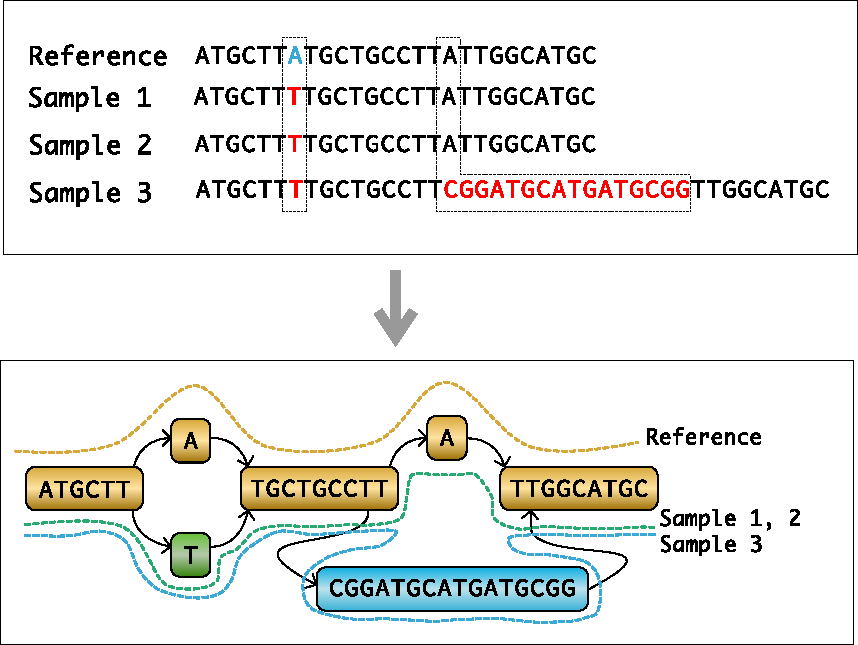
\includegraphics[width=0.8\textwidth]{intro/fig4.pdf}
        \vspace{3mm}
        \caption[Graph-based pangenome approach]{\textbf{Graph-based pangenome approach.} \\
        \footnotesize{\textbf{(a)} The majority of the pangenome studies follow the classical pangenome approach, where multiple linear genomes are compared without compressing redundant information and might lack orthology relationships. \textbf{(b)} Graph-based pangenome approach offers unified and richer multiple genomes representation. Nodes contain DNA sequences and nodes with continuous sequences connected with directed edges. Redundant information across genomes is compacted by collapsing invariant regions into a single node. Alternative nodes in the bubbles (green and blue nodes) are alleles in the population. Thus, graphs allow sequence comparison to occur in the context of variations. Walks through the graph might retrace the original sets of sequences from which it was built (dashed line).}}
        \label{fig14:graph}
\end{figure}



\subsection{Graph genomes implementations}

The first pangenome graph implementation was based on the DBG (\emph{De Bruijn Graphs}). Sequencing reads from all samples were fragmented into $k$-mer length $k$, and the graph was constructed by inducing the first and second node where $k-1$ bp end of first node that overlap with the $k-1$ bp start of the second node. Nodes are “coloured” where each colour map to the origin of the samples. \citet{iqbal2012novo} developed \emph{Cortex}, a coloured DBG-based pangenome tool. They used it to construct a population graph from 164 human samples and identified 3.2 Mb novel sequences that are absent in the human reference genome. Because the genomic coordinates are discarded by fragmenting the reads, DBG-based approaches are not suitable for resequencing study, although a recent study attempts to embed a long-range path information into the graph \citep{turner2018integrating}. 

Current well-established graph genome implementations establish a variation graph as an extension of the linear reference genome \citep{eggertsson2017graphtyper,garrison2018variation,sibbesen2018accurate,rakocevic2019fast,kim2019graph}. This implementation utilizes the existing linear reference genome as a backbone, which is then augmented with known variants. To build the graph, reference sequences are split at variable sites, and variants are added as alternative nodes of the reference bases in the graphs. The linear reference coordinates are embedded in the graphs as a path, and the nodes are referred to relative to this reference path. Thus, the reference path provides a stable coordinate system that can be used as a basis for alignment and annotation \citep{garrison2018variation}. 


\emph{Graphtyper }is the first open-source variation graph-based software designed for genotyping from a local (region-specific) graph \citep{eggertsson2017graphtyper,eggertsson2019graphtyper2}. It uses a variant file (\emph{VCF}) as input source of variant sites and a reference assembly as backbone of the graph. Because of the limited variations modelled by a VCF file, the output graph is directed and acylic containing insertions and deletions but not necessarily complex variations (Fig. \ref{fig15:mut}b). \emph{Graphtyper} applies a two-step genotyping proces. The  “discovery step” is similar to linear reference-guided variant analysis. Sequencing reads are mapped to the linear genome and variants are identified from the alignments. This step is then followed by read realignment towards local graphs. To this end, \emph{Graphtyper} first constructs small regional graphs of 10 kb windows that are subsequently augmented with variants discovered during the first step. Then, \emph{Graphtyper} extracts reads that were initially mapped by the linear mapper, realigns them onto the local graph and performs the variant genotyping from the refined alignments. This approach does, however, not  fully  eliminate reference bias because it relies on the global read placement by a linear mapper. However, this design makes it highly efficient as evidenced with scalable joint genotyping of close to 50,000 Icelander samples \citep{eggertsson2019graphtyper2}. Additionally, Graphtyper outperformed current state-of-the-art linear genome-based tools (e.g., \emph{SAMtools} and \emph{GATK}), particularly from more refined variants surrounding Indels with considerably reduced Mendelian errors \citep{eggertsson2017graphtyper}.

\begin{figure}[!htb]
    \centering
    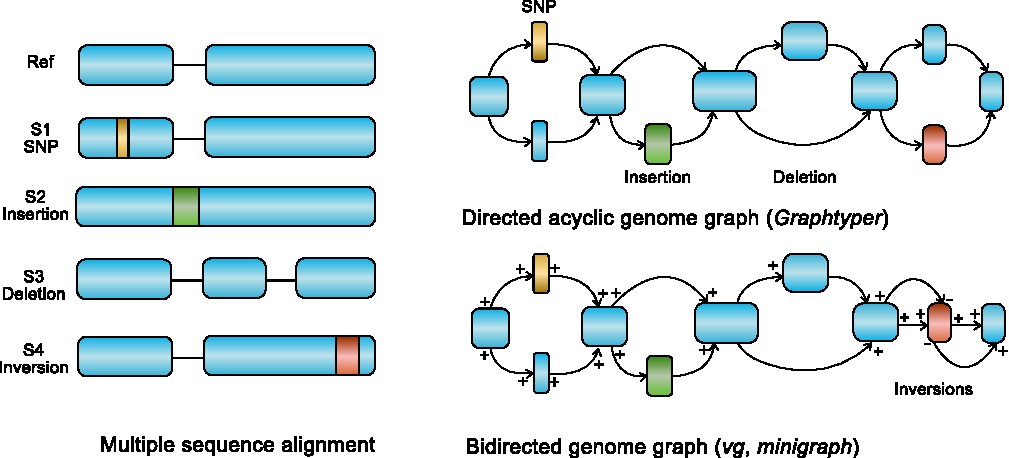
\includegraphics[width=0.9\textwidth]{intro/fig5.pdf}
        \vspace{3mm}
        \caption[Genetic variant representation in the genome graphs]{\textbf{Various genome graph implementations and representations of variations in the graphs} \\
        \footnotesize{\textbf{(a)} multiple sequence alignments capturing sequence relationships. \textbf{(b)} directed genome graphs underlying the data structure of Graphtyper, similar to multiple sequence alignments but with compressing redundant information. \textbf{(c)} general bidirected sequence graph as implemented in vg that each edge endpoint has independent orientation. Note  forward (+) and reverse strand (-) to indicate inversions (orange). Figures are adapted from \citep{eizenga2020pangenome}.}}
        \label{fig15:mut}
\end{figure}

\subsection{Construction of the whole-genome variation graphs with the \emph{vg toolkit}}

The variation-graph toolkit (\emph{vg}) is the first open-source toolkit designed to perform the full suite of genome analyses from genome graphs in species with a gigabase-sized genome \citep{garrison2018variation}. The basic structure of \emph{vg} is a bidirected sequence graph that can express the strand-ness of the input sequences (Fig. \ref{fig15:mut}c). Each edge endpoint has an independent orientation to indicate whether the forward or reverse sequences are spelled out when visiting the node \citep{paten2017genome}. Therefore, \emph{vg} can represent variations with complex topology e.g., inversion or translocation. Haplotype information from the sample are stored in an index so that analysis from the graph can consider haplotype information \citep{siren2020haplotype}. Graph mapping in \emph{ vg} is optimized for short–sequencing reads that follows the seed-and-extend paradigm. It relies on a \emph{GCSA2 }graph index (a generalization of linear genome-based\emph{ BWT} index to graphs) for a fast seed query \citep{siren2017indexing}. The index construction is the computationally most demanding step because all $k$-bp paths in the graphs need to be enumerated, which is intractable in complex regions with high variant density. In practice, \emph{vg} can handle complex region by indexing on a simplified graph e.g., retaining only biologically plausible paths informed by the haplotype index \citep{siren2017indexing}. Graph mapping is computationally more expensive than linear mapping because multiple alternative paths need to be explored. To make graph-based mapping competitive to linear mapping, \emph{vg mapper} is currently being improved to utilize minimizer-based mapping paradigm and restrict the mapping that conforms the haplotype paths. It can achieve the same mapping speed as the \emph{BWA} linear mapper with more accurate alignment performance, especially for structural variant genotyping \citep{siren2020genotyping}. 

\emph{To be continued with more comments}


\singlespacing
\footnotesize

% uncomment so that references appear on the same page
% \let\Origclearpage\clearpage
% \let\clearpage\relax


\bibliographystyle{abbrvnat}
\bibliography{references/introduction}
%\printbibliography[title=References]

% \let\clearpage\Origclearpage

\ifdefined\BuildingFromMainFile
\else
   \end{document}
\fi